\csname documentclass\endcsname[../main.tex]{subfiles}
\graphicspath{{\subfix{../images/}}}
\begin{document}

This section will present the project’s results, evaluate them, and discuss the findings. We will first focus on evaluating the predictive models’ performance before reviewing the outcomes of the traffic simulations and congestion management strategies. Finally, we will finish with a detailed discussion of the findings and limitations.

\subsection{Model Performance Evaluation}
This first results section evaluates the predictive models created and their variations. We present the results of the three models implemented, including metrics, visualisations and a discussion.

\paragraph{ARIMA Model}
\label{link:arima-results}
This model was abandoned from our final prototype after disappointing results due to its insufficient complexity for our purposes. The results of the ARIMA forecast on the test sensor are shown in \fig{arima-result}. The plot shows the actual traffic speed split by train and test data, with the forecast in the red dashed line. As can be seen, the fluctuations present in the traffic data are too complex for the ARIMA model, resulting in the model simply constantly fitting the mean of the data as its output. This is a disappointing result; however, it is expected as the ARIMA model uses only the traffic data and pure timestamps to fit the model. This is just too complex for our purposes and was, therefore, abandoned.

\begin{figure}[!ht]
  \centering
  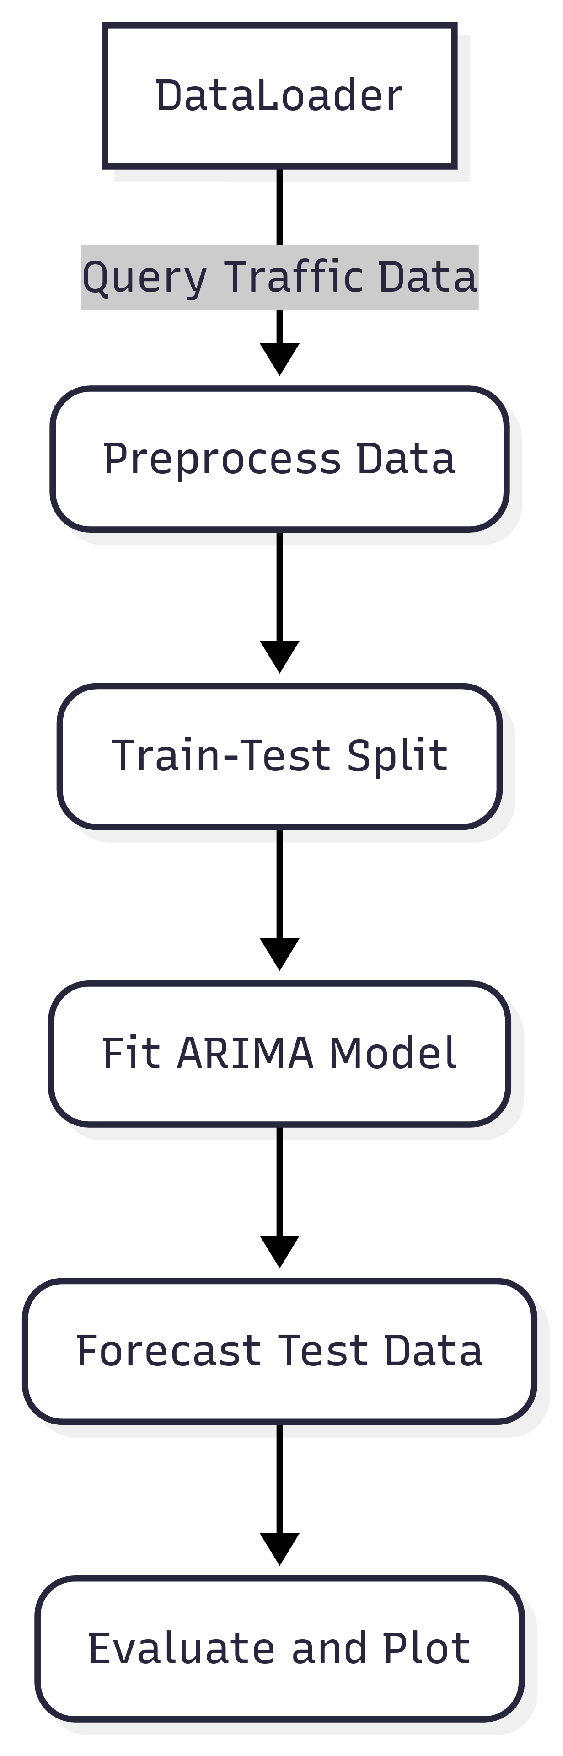
\includegraphics[width=\textwidth]{images/results-discussions/arima.pdf}
  \caption{Plot of ARIMA model forecast results compared with test data}
  \label{fig:arima-result}
\end{figure}

\paragraph{LSTM Model}
\label{link:lstm-results}
The LSTM model showed interesting results that were expected, as previously discussed. We hypothesised that the LSTM would work exceptionally well for short-term but not long-term forecasting. This is precisely what our results show. \fig{lstm-1-state} shows a plot of the actual vs predicted traffic speed from the LSTM model in a one-step forecast, meaning the model predicts one timestep ahead from the current real one, and this is performed for all data points. \fig{lstm-walk}, on the other hand, shows the same Plot but with a walk-forward forecast, where the model attempts to predict the speed 100 timesteps into the future based on the previous prediction. Please note that these plots use scaled speed instead of real speed. The results are clear: the LSTM model performs exceptionally well for short-term forecasting, showing a precise following of the real traffic curve in our results.
On the other hand, this model becomes unusable for long-term forecasting, as shown in the results of the walk-forward forecast. The forecast initiates at the same speed level. However, it quickly diverges from the real data as it loses any understanding of the data, multiplying the errors of each time step. This model was also abandoned as we focus on long-term forecasting as explained in the \textbf{\hyperref[link:model-decision]{model decision}} section.

\begin{figure}[!ht]
  \centering
  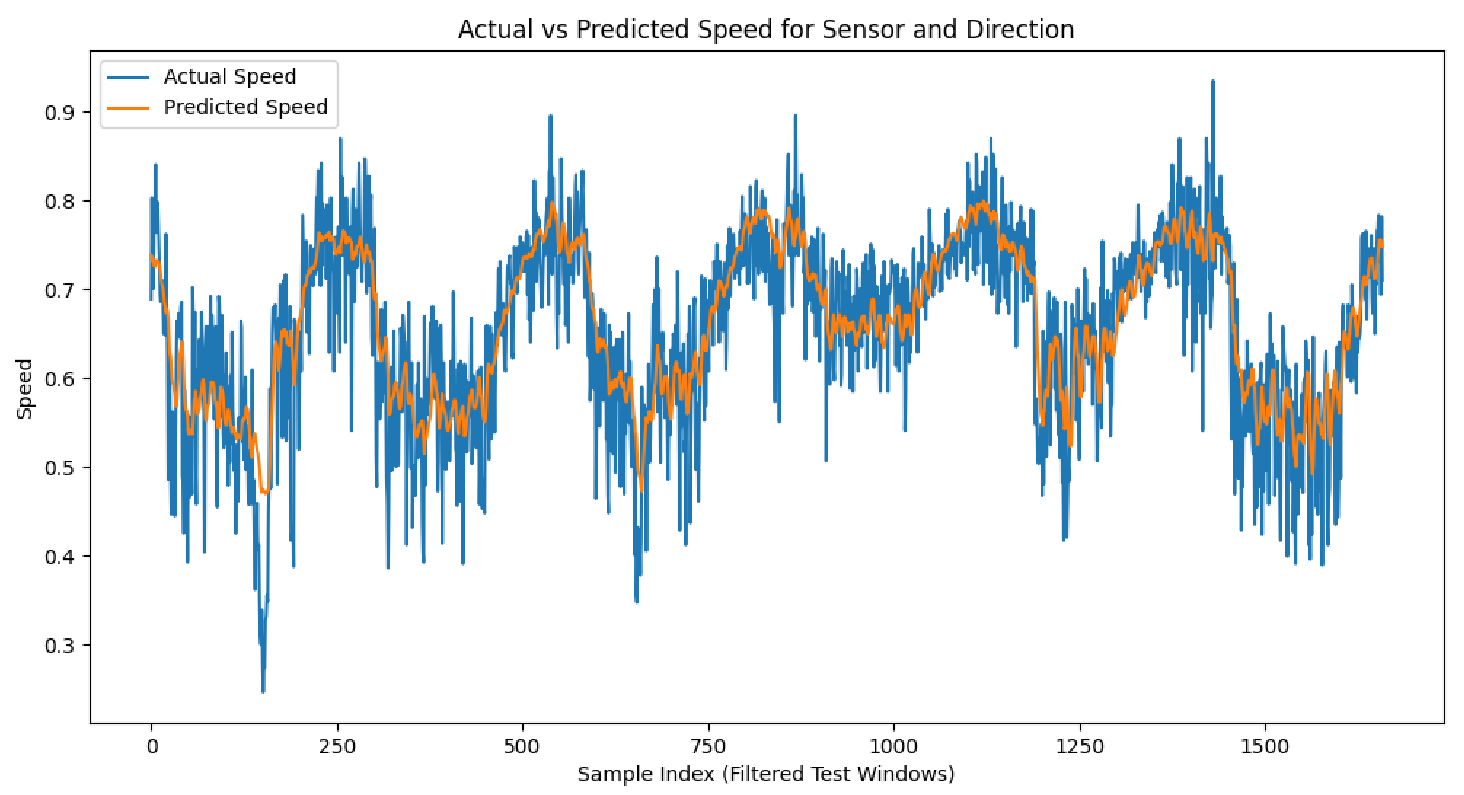
\includegraphics[width=\textwidth]{images/results-discussions/1-state-predictions.pdf}
  \caption{Plot of LSTM model one-step forecast results compared with test data}
  \label{fig:lstm-1-state}
\end{figure}

\begin{figure}[!ht]
  \centering
  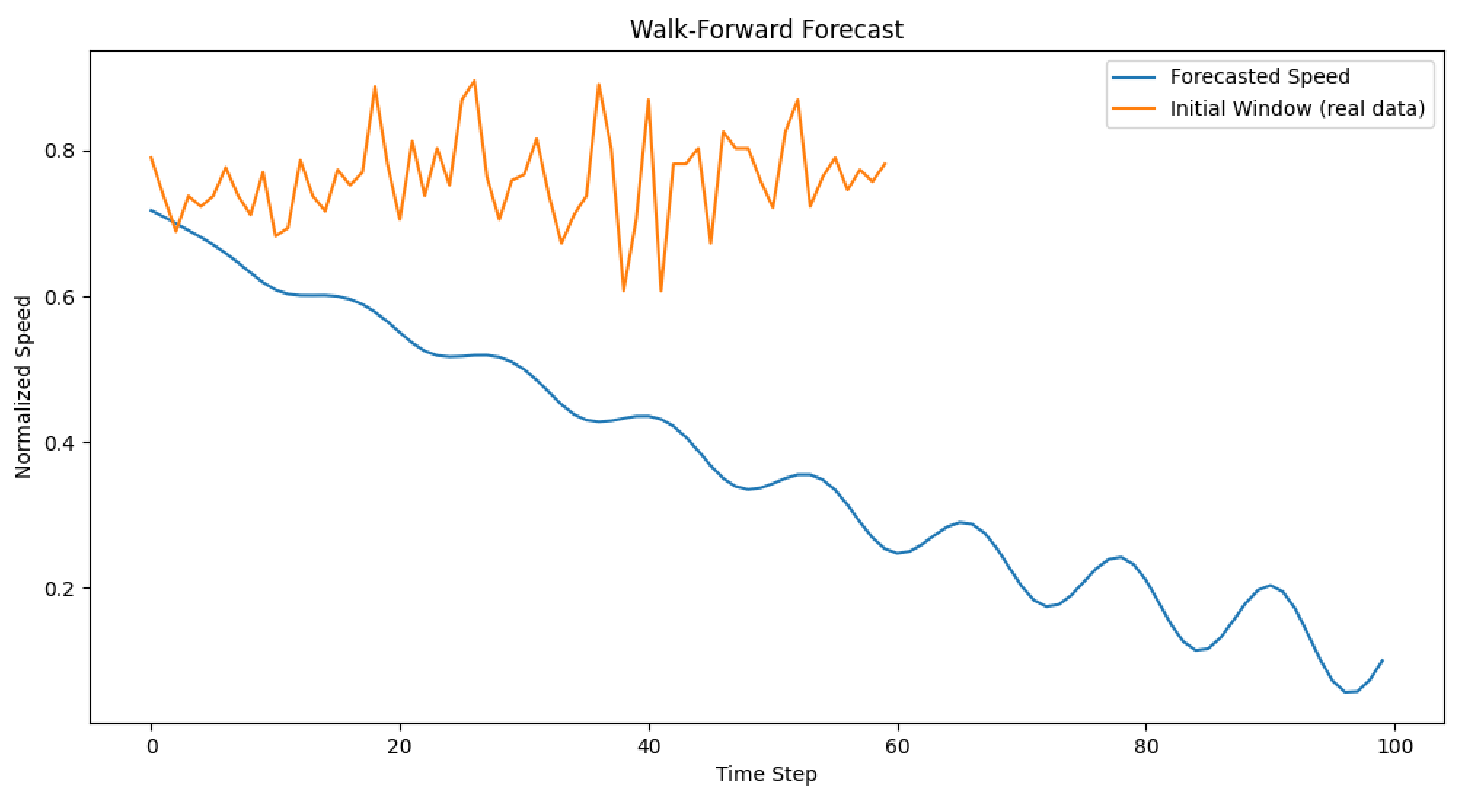
\includegraphics[width=\textwidth]{images/results-discussions/walk-forward.pdf}
  \caption{Plot of LSTM model walk-forward forecast results compared with test data}
  \label{fig:lstm-walk}
\end{figure}

\paragraph{MLP Model}
Our final MLP Model performed exceptionally well, especially after fine-tuning. It was able to model the complex time features and the impact of events, furthering the model's prediction accuracy. In the next section, we will go into more detail about the features used in this final model, while we present the final model performance results here. \fig{mlp-with-events} shows plots of the final MLP model on the test sensor. These show the performance of the model’s predictions compared with the actual data for the whole test data period. The plot is split into three, showing the whole timeline and the middle ten and three per cent to zoom into specific trends. Looking at the middle 3 per cent, we can see the model performs very accurate predictions, following the curve of actual results along the time axis, further confirmed by the middle 10 per cent plot. Looking at the whole timeline is where we can understand the impact of events. Many sharp declines can be seen throughout the timeline, where events were happening around the area and where the model predicted sharper traffic speed declines due to this. We can see these follow the actual data, with the sharp declines coinciding with the ones in the actual data, although at a grander scale. 

Overall, the predicted traffic closely tracks the ground truth, with minimal error during peak and off-peak periods, presenting a robust model for predictions. The results of this model are provided in \tab{model_results}. This table provides the errors of the same test data set, as shown in the Plot and the average errors of training on all available, consistent sensors. For this, we trained all sensors as we described in the design, resulting in 63 sensor-direction combinations of models trained to predict the speed data. 

\begin{table}[!ht]
    \centering
    \caption{MLP Model Performance Metrics}
    \label{table:model_results}
    \resizebox{0.8\textwidth}{!}{%
    \begin{tabular}{lcccc}
        \toprule
        \multirow{2}{*}{\textbf{Model}} & \multicolumn{4}{c}{\textbf{Metrics}} \\
         & \textbf{MAE (MPH)} & \textbf{MSE (MPH)\sus{2}} & \textbf{RMSE (MPH)} & \textbf{MAPE (\%)} \\
        \midrule
        Test Sensor (drakewell-1163-nw)       & 2.83 & 14.49 & 3.81 & 11.47 \\
        Average of All Sensors  & 2.32 & 15.85 & 3.98 & 12.44 \\
        \bottomrule
    \end{tabular}
    }
\end{table}

The results in metrics are also highly encouraging. For sensors where speed hovers around the speed limit (30 MPH), an average MAE of 2.32 MPH and RMSE of 3.98 indicate a low prediction error, corresponding to less than 12.5\% deviation on average. This suggests that the model can accurately capture typical traffic speed patterns in free-flow conditions. These error values are sufficiently low to support real-time traffic monitoring and early detection of slowdowns, as even minor deviations from the free-flow speed can reflect emerging congestion. We will further compare these results in the \textbf{\hyperref[sec:conclusions-future]{conclusions}} against other works using MAPE.

\begin{figure}[!ht]
  \centering
  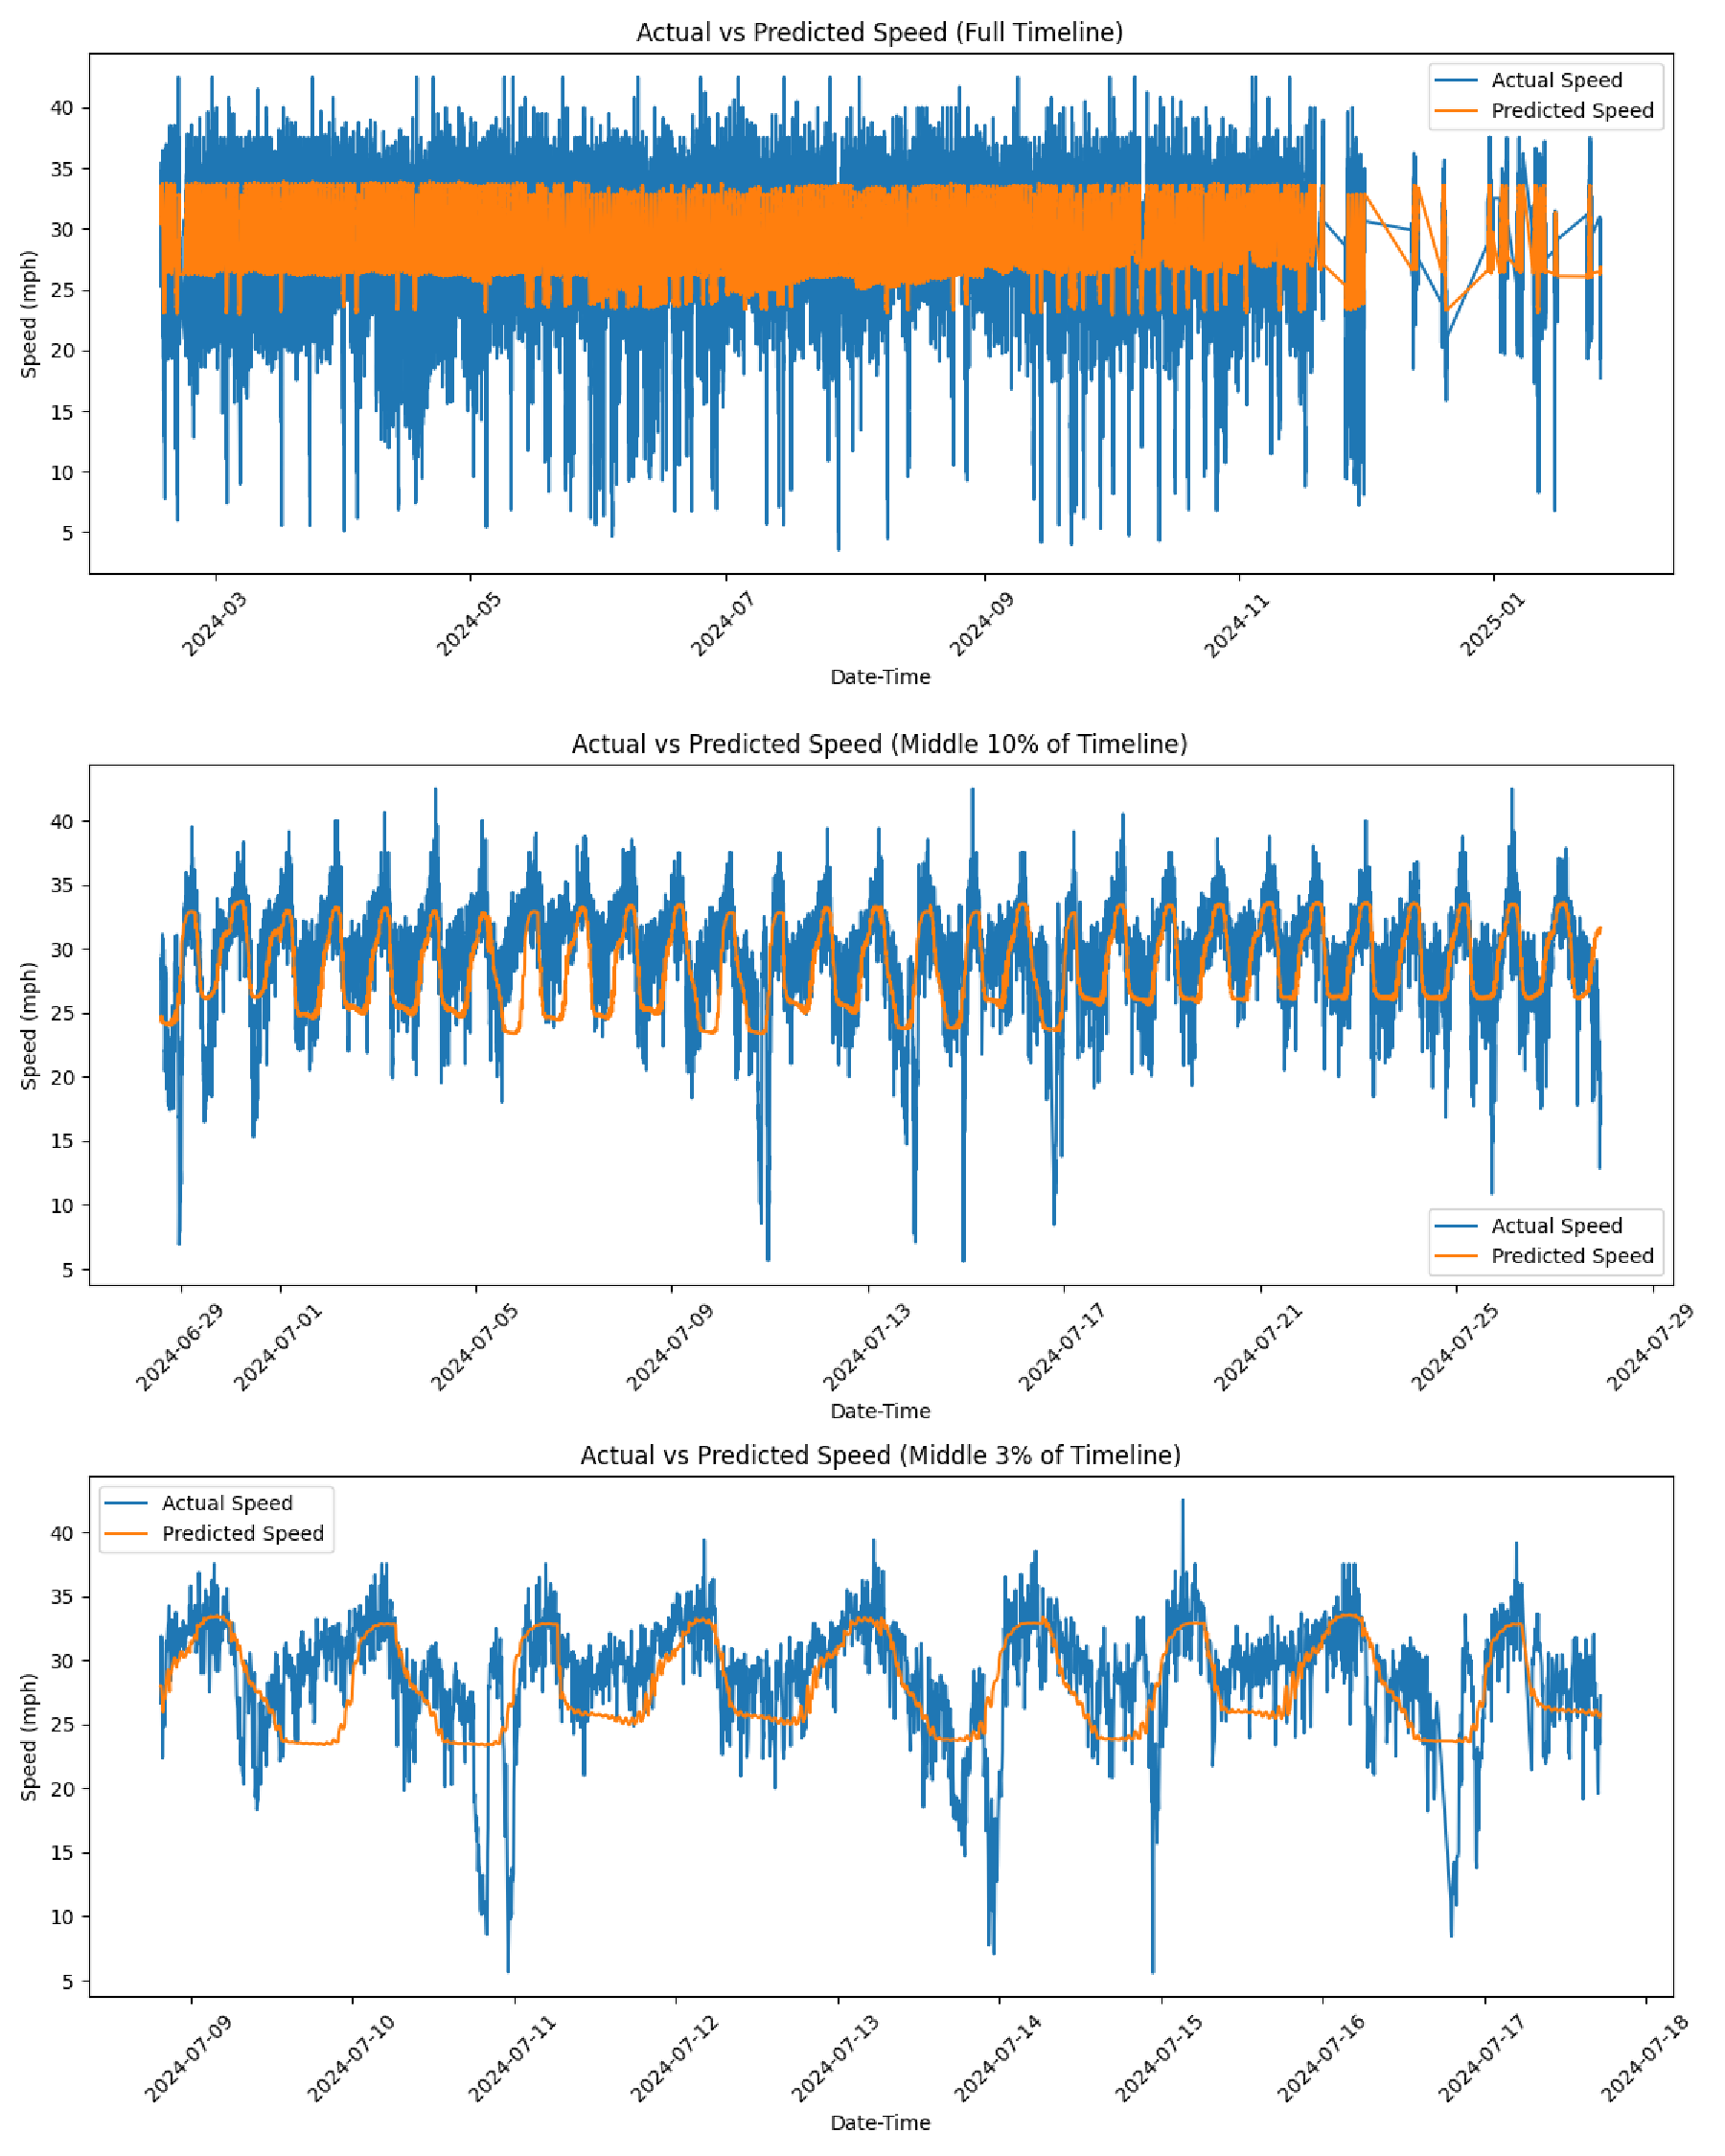
\includegraphics[width=\textwidth]{images/results-discussions/mlp-with-events.pdf}
  \caption{Plot of MLP model forecast results compared with test data at three zoom levels}
  \label{fig:mlp-with-events}
\end{figure}

\paragraph{Model Decision and Discussion of Results}
\label{link:model-decision}
The ARIMA model was abandoned as it was simply unsuitable for our purposes. The LSTM model was also abandoned, as while the short-term forecasting capabilities were excellent, these were just too short-term for our purposes, and the long-term forecasting was disappointing. We decided on the MLP model that showed excellent results, a good integration of extra features, and the capability of long-term forecasting that is superior to short-term forecasting, as it provides a broader window for proactive intervention as well as strategic planning:
\begin{enumerate}
    \item For our purposes, a long-term forecast allows for proactive interventions to occur much earlier if needed.
    \item Long-term forecasting learns trends and the impact of features compared to heavily relying on the last measurement. These can provide sustained improvements over a longer period.
    \item These forecasts allow for advanced warnings and observability, even for human operators. When considering using a predictive model outside of automatic congestion management, long-term observability and warning can be incredibly useful for human operators to plan and allocate resources effectively.
    \item Long-term forecasting can be made more computationally efficient, as it can be run in the background in the cloud or fog layer a long time in advance, compared to short-term forecasting that might need to run locally and needs to be run at the moment.
\end{enumerate}

\subsubsection{Hyperparameter Tuning}
We briefly describe the results of the hyperparameter tuning run for the MLP Model. The resulting optimal architecture is shown in \tab{mlp_architecture_details}. The architecture derived from the optimisation is quite deep, with four layers, showing a preference for a deeper network to derive more complex patterns from our features. Another point to note is that the dropout rates vary to balance regularisation but are higher towards the initial layers, lowering as the network becomes deeper. One final note is the consistent use of ReLU activation, which is consistent with typical uses in deep networks, as it prevents the vanishing gradient problem.

\begin{table}[!ht]
\centering
\caption{MLP Tuned Architecture}
\label{table:mlp_architecture_details}
\resizebox{0.45\textwidth}{!}{%
\begin{tabular}{cccc}
\toprule
\textbf{Layer} & \textbf{Units} & \textbf{Activation} & \textbf{Dropout} \\
\midrule
Input Layer    & 96   & ReLU    & 0.3 \\[0.5ex]
Hidden Layer 1 & 256  & ReLU    & 0.2 \\[0.5ex]
Hidden Layer 2 & 256  & ReLU    & 0.1 \\[0.5ex]
Hidden Layer 3 & 96   & ReLU    & 0.3 \\[0.5ex]
Hidden Layer 4 & 256  & ReLU    & 0.0 \\[0.5ex]
Optimiser      & -    & RMSprop & -   \\[0.5ex]
\bottomrule
\end{tabular}%
}
\end{table}

\subsubsection{Feature Engineering Comparison and Impact}
In this section, we delve deeper into the MLP model results. More specifically, we focus on comparing the impact of different features and the features used for the final model. \tab{feature_performance_comparison} shows the results of training the test sensor model with different combinations of features and their performance. Our baseline model is the MLP with basic time encoding (Model ID 0), achieving a MAE of 2.90, RMSE of 4.23 and MAPE of 12.70\%. With feature engineering effort, and most importantly, through our encoding of events in the model, we managed to bring this down to a MAE of 2.83, RMSE of 3.81, and MAPE of 11.47\%, resulting in our final model (Model ID 3), using only cyclic time encoding and our custom event encoding. We delve into feature importance and impact in more detail below.

\begin{table}[!ht]
\centering
\caption{MLP Feature and Performance Comparison}
\label{table:feature_performance_comparison}
\resizebox{\textwidth}{!}{%
\begin{tabular}{ccccccccccc}
\toprule
\textbf{Model ID} & \textbf{Basic Time} & \textbf{Cyclic Time} & \textbf{Binary Event} & \textbf{Custom Event} & \textbf{LLM Estimations} & \textbf{Weather} & \textbf{MAE (MPH)} & \textbf{MSE (MPH)\sus{2}} & \textbf{RMSE (MPH)} & \textbf{MAPE (\%)} \\
\midrule
0 & $\checkmark$ & & & & & & 2.90 & 17.89 & 4.23 & 12.70 \\[0.5ex]
1 & & $\checkmark$ & & & & & 2.85 & 17.27 & 4.16 & 12.47 \\[0.5ex]
2 & & $\checkmark$ & $\checkmark$ & & & & 2.88 & 16.57 & 4.07 & 12.15 \\[0.5ex]
3 & & $\checkmark$ & & $\checkmark$ & & & 2.83 & 14.49 & 3.81 & 11.47 \\[0.5ex]
4 & & $\checkmark$ & & $\checkmark$ & $\checkmark$ & & 2.84 & 16.78 & 4.10 & 12.33 \\[0.5ex]
5 & & $\checkmark$ & & $\checkmark$ & & $\checkmark$ & 2.88 & 16.36 & 4.05 & 12.27 \\[0.5ex]
\bottomrule
\end{tabular}%
}
\end{table}

\paragraph{Time Encoding}
As discussed previously, we tested two designs of time feature encoding: basic and cyclic. As shown in the results table, this switch can improve performance slightly (\~{}3.5\% in RMSE and \~{}0.2\% in MAPE). We verify our hypothesis that the cyclic encoding can better model these features as continuous and, therefore, help the model understand the trends of time features. We can visualise this difference in the figures below. \fig{non-cyclic} shows the model predictions using basic time encoding (Model ID 0), while \fig{cyclic} shows the model predictions using cyclic time encoding (Model ID 1). Using the basic time encoding, we can see the build-up and break of the time features continuously over the whole timeline, while the cyclic encoding flows continuously.

\begin{figure}[!ht]
  \centering
  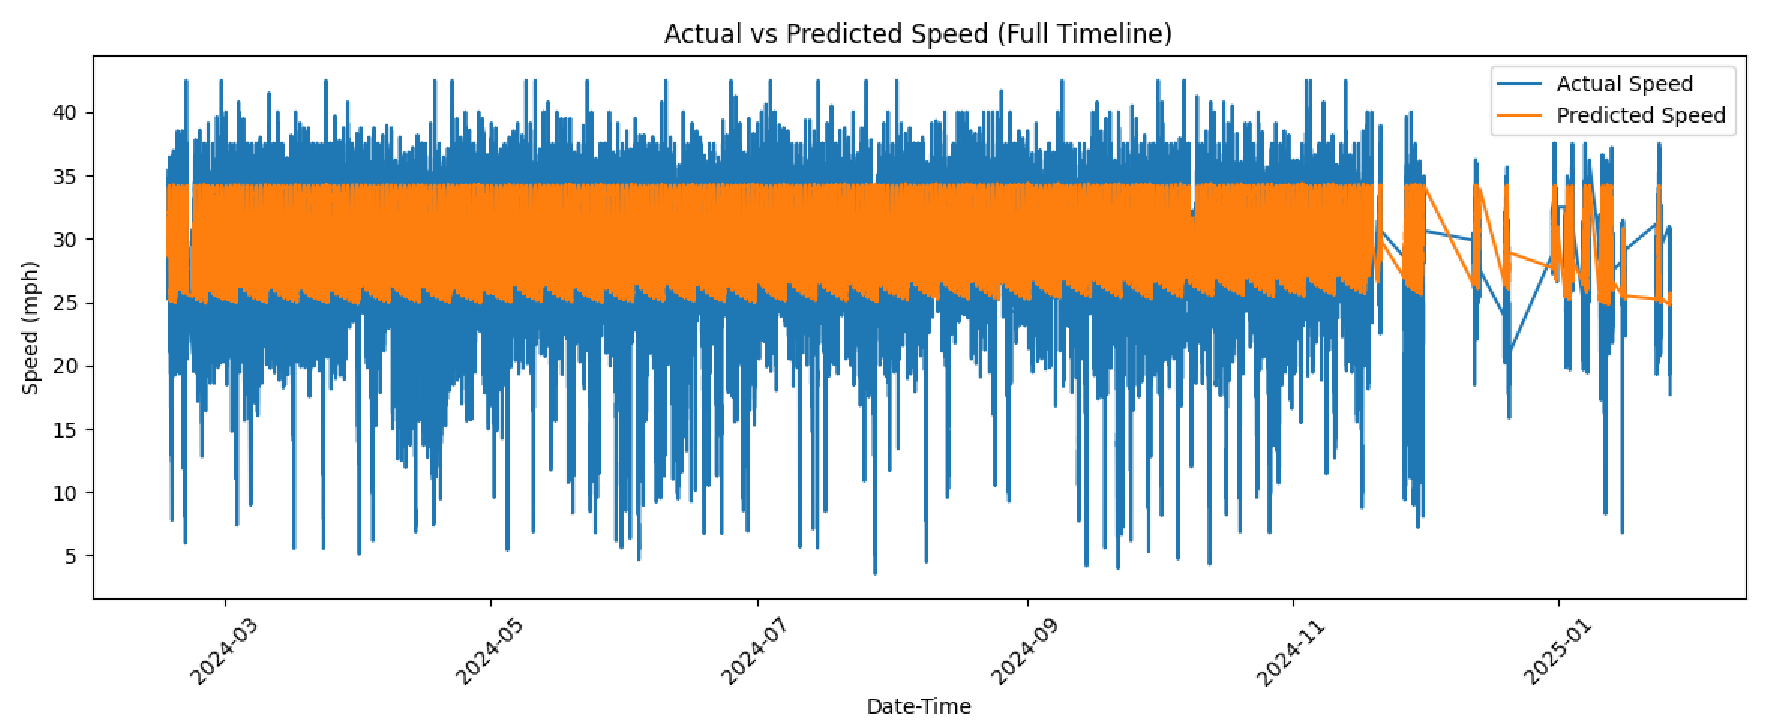
\includegraphics[width=\textwidth]{images/results-discussions/non_cyclic.pdf}
  \caption{Plot of MLP model forecast results compared with test data using basic time encoding}
  \label{fig:non-cyclic}
\end{figure}

\begin{figure}[!ht]
  \centering
  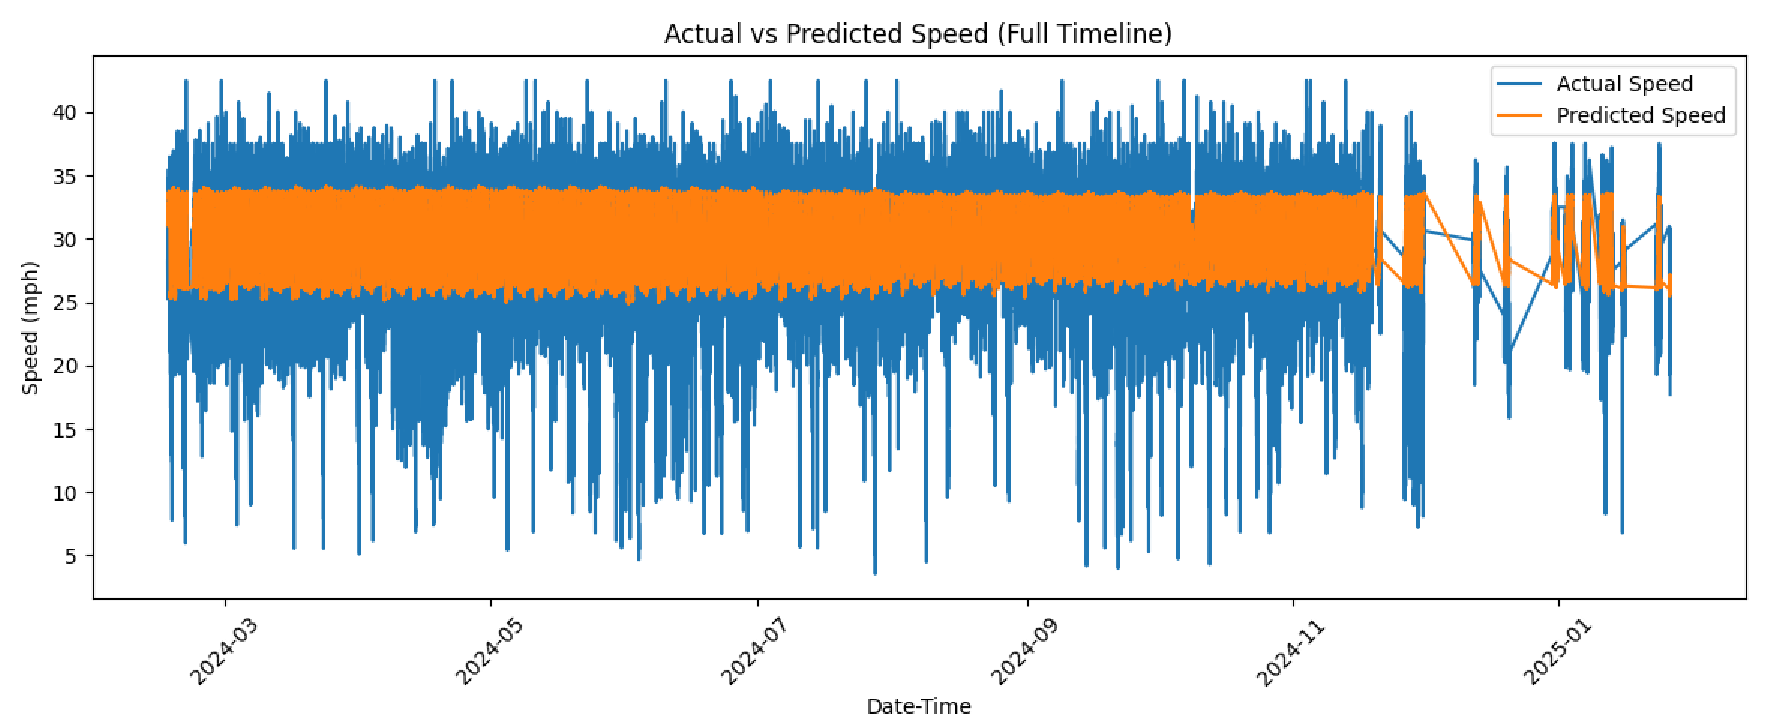
\includegraphics[width=\textwidth]{images/results-discussions/cyclic.pdf}
  \caption{Plot of MLP model forecast results compared with test data using cyclic time encoding}
  \label{fig:cyclic}
\end{figure}

\paragraph{Weather Features}
As discussed previously, we tested adding weather features to our model, as weather can seriously impact traffic congestion. The results of adding these features are in Model ID 5, with a MAPE of 12.27\% and a RMSE of 4.05. This is considerably worse performance compared to the same model without weather features (Model ID 3), which had a MAPE of 11.47\% and RMSE of 3.81. Our hypothesis of why the performance decreased with the added weather features is twofold:
\begin{itemize}
    \item Our weather data source may not be accurate enough to present useful features. Open-Meteo provides weather data correct to the nearest kilometre and hour. Since weather-impacting traffic can sometimes be particular to a location and time, this may not be of enough resolution to impact our model.
    \item Our MLP architecture may not be deep enough to enable a deeper understanding of the weather impact. A deeper network or different architecture may be required to use weather features.
\end{itemize}

\paragraph{Event Features}
Event features were by far the most important features for our model predictions, further confirming the validity and usefulness of this project. We tested three different architectures for this: binary encoding, custom encoding, and custom encoding with the added LLM Estimations. \fig{binary-events} shows the model predictions using binary event encoding (Model ID 2), \fig{events} shows the model predictions using custom event encoding (Model ID 3), and \fig{llm} shows the model predictions using custom event encoding combined with LLM Attendance Estimation (Model ID 4). Introducing binary event encoding improved accuracy by \~{}0.3\% in MAPE and \~{}2\% in RMSE. This improvement is significant, especially in RMSE, which is coherent with our expectations. MSE and RMSE give higher importance to the peaks and dips of predictions, where the impact of event features lies. \fig{binary-events} clearly shows the impact of events on the predictions, leading to the more significant dips seen during events. Using our custom event encoding, we see an even more considerable improvement of \~{}1\% in MAPE and of \~{}8.8\% in RMSE, compared to no event features. \fig{events} shows the visualisation of this effect, where the encoding allows the model to differentiate the magnitude of dips according to the event type and time. These results prove the impact of our custom event encoding in significantly improving the accuracy of predictive models in traffic engineering.

Finally, we tested our LLM-based Attendance Estimation feature. However, the results were disappointing as they decreased the accuracy compared to the custom event encoding alone. Future work would be required to explain the exact cause; however, our hypothesis is the following:
\begin{itemize}
    \item The Event Type features already present in our custom event encoding are sufficient for the model to understand attendance by differentiating between matches and concerts.
    \item The venues we focus on in this project are large venues where events usually fill them. Therefore, the attendance estimation is of less importance as the venue itself is characteristic of the attendance.
    \item Once again, our model architecture might not be deep enough for this type of feature to be useful. The visualisation (\fig{llm}) shows that adding this feature breaks the model as the event peaks are no longer present, and some predictions are lost.
\end{itemize}

\begin{figure}[!ht]
  \centering
  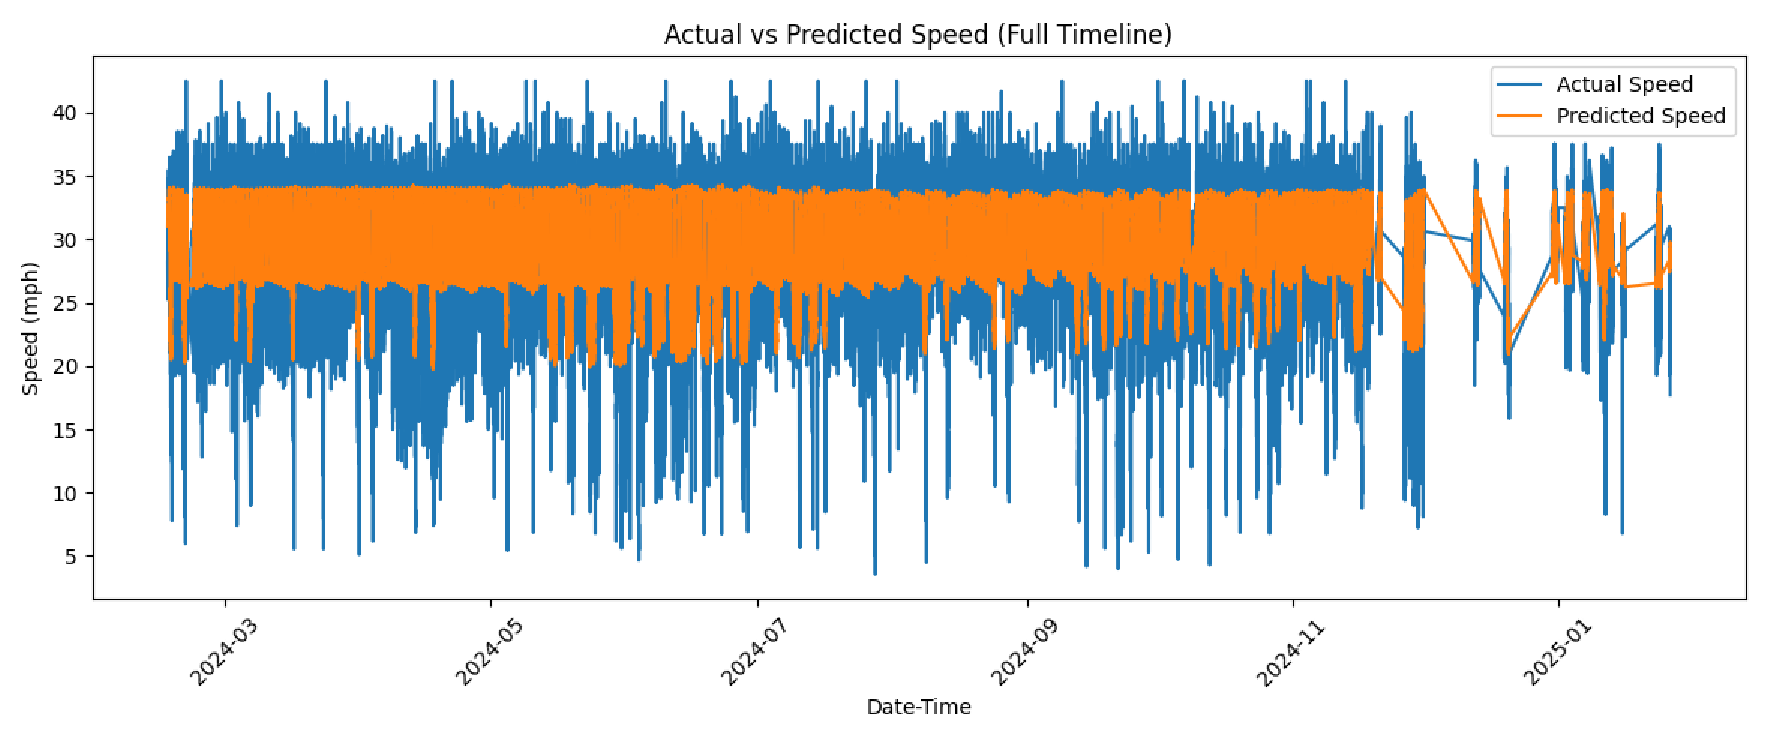
\includegraphics[width=\textwidth]{images/results-discussions/binary-events.pdf}
  \caption{Plot of MLP model forecast results compared with test data using binary event encoding}
  \label{fig:binary-events}
\end{figure}

\begin{figure}[!ht]
  \centering
  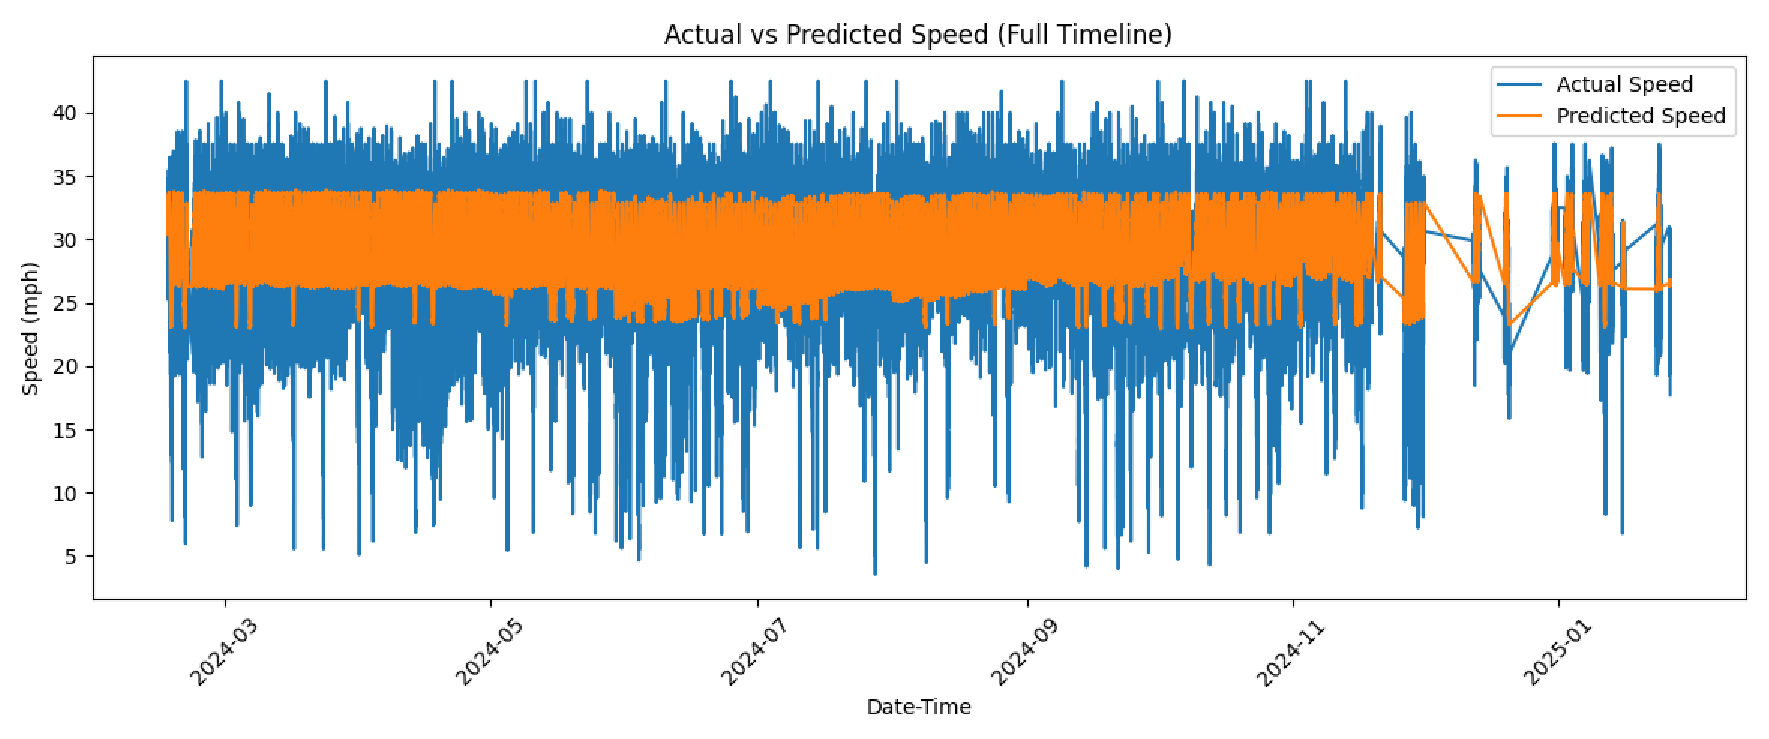
\includegraphics[width=\textwidth]{images/results-discussions/events.pdf}
  \caption{Plot of MLP model forecast results compared with test data using custom event encoding}
  \label{fig:events}
\end{figure}

\begin{figure}[!ht]
  \centering
  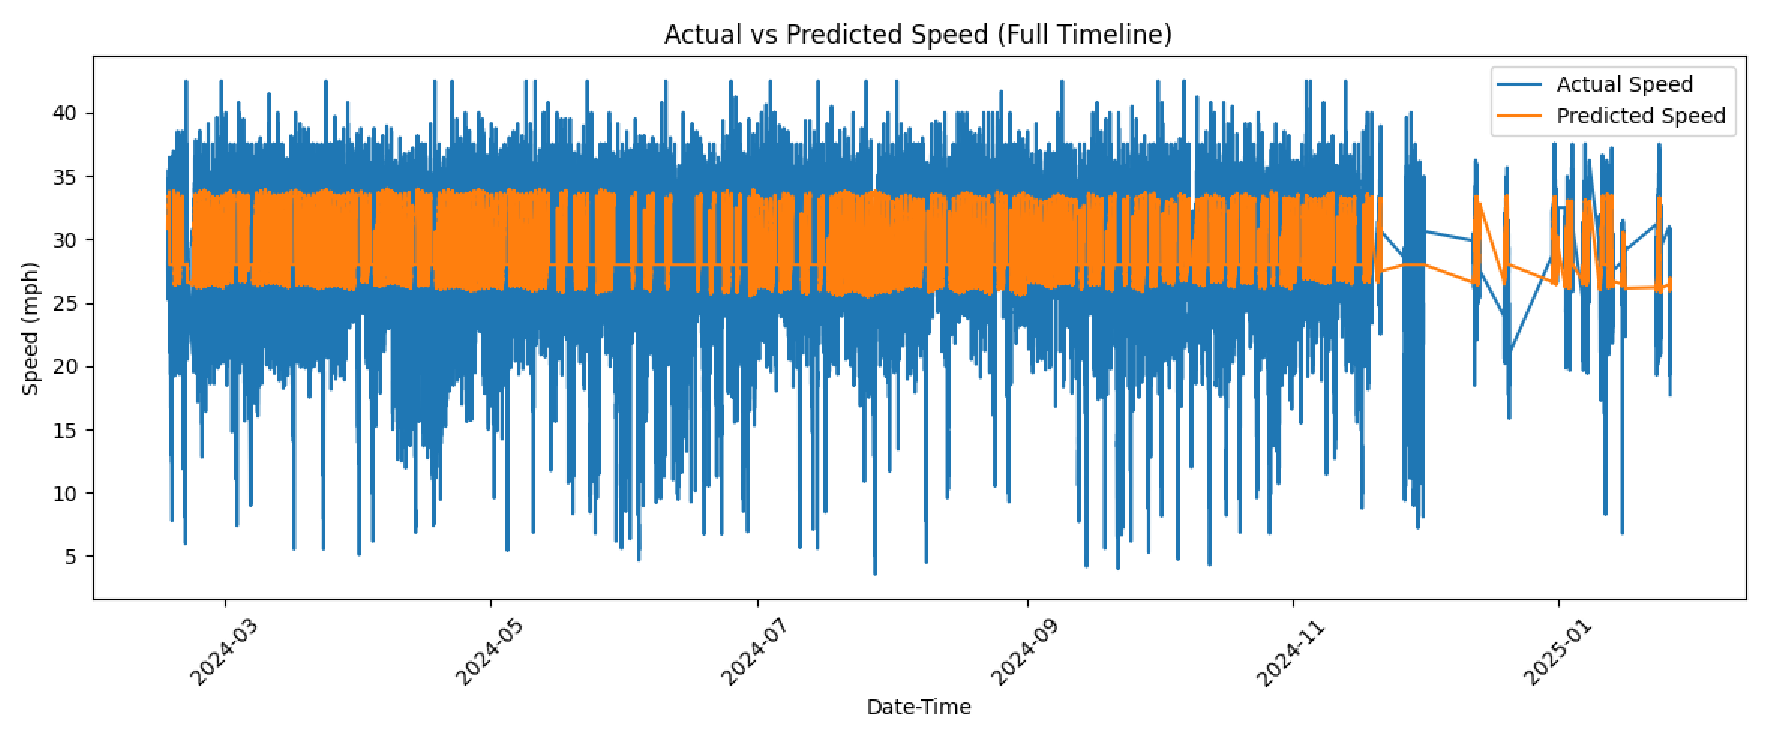
\includegraphics[width=\textwidth]{images/results-discussions/llm.pdf}
  \caption{Plot of MLP model forecast results compared with test data using LLM estimation}
  \label{fig:llm}
\end{figure}

\subsection{Simulation Outcomes}
In this section, we will delve into the results and discussion of the simulations. We start with real-world demand generation results to understand the accuracy level of the simulated scenarios. We then move on to some quick results of the reactive scenarios’ hyperparameter choices, which allowed us to set the reactive rule hyperparameters used for the simulation run. After this, we showcase the simulation results, comparing the different strategies and demonstrating the effectiveness of our proactive techniques using predictions.

\subsubsection{Real-World Demand Generation Results}
\label{link:demand-results}
Firstly, we cover the results of our demand generation technique for simulation. This allows the understanding of the validity of the results through the accuracy of the simulated scenarios they are run in. \tab{demand-results} shows the results of the errors in the simulated scenarios, comparing the gold standard (the actual speed data collected) with the results of the induction loop sensor data fed back from the simulation. We present the results of a typical and event day for a single data point, which we plot for visualisation, as well as the average over all sensors and simulation days.

\begin{table}[!ht]
    \centering
    \caption{Real-World Demand Generation Error Metrics}
    \label{table:demand-results}
    \resizebox{0.75\textwidth}{!}{%
    \begin{tabular}{lcccc}
        \toprule
        \multirow{2}{*}{\textbf{Simulation}} & \multicolumn{4}{c}{\textbf{Metrics}} \\
         & \textbf{MAE (MPH)} & \textbf{MSE (MPH)\sus{2}} & \textbf{RMSE (MPH)} & \textbf{MAPE (\%)} \\
        \midrule
        Typical Day (2024-04-15)       & 2.39 & 11.67 & 3.42 & 8.13 \\
        Event Day (2024-05-04)  & 3.87 & 23.67 & 4.87 & 18.48 \\
        Typical Days Average  & 3.71 & 31.66 & 5.63 & 12.61 \\
        Event Days Average  & 3.94 & 30.60 & 5.53 & 19.13 \\
        \bottomrule
    \end{tabular}
    }
\end{table}

Given the challenge of simulating demand through traffic count and comparing the observed speed, these results are minimally encouraging. While, on average, the errors are pretty high (12.61\% for typical days and 19.13\% for event days), the trend is the most important aspect of simulated demand for our purposes. \fig{demand-normal} shows a plot of the actual real-world speed compared with the observed in simulation for our test sensor on a typical day, and \fig{demand-event} for an event day. These show that our simulated demand follows the curve closely at a lower overall speed level. This results from scaling down the demand to prevent total network congestion. As such, while the metric errors are relatively high, we are still confident that the demand generated is sufficiently close to the real world to provide results. For the event day demand, this also confirms our concern with count-based demand generation, where it struggles to model the sudden peaks and drops of speed during events, further evidenced by the higher MAPE. We will discuss this in more detail in the following section.

\begin{figure}[!ht]
  \centering
  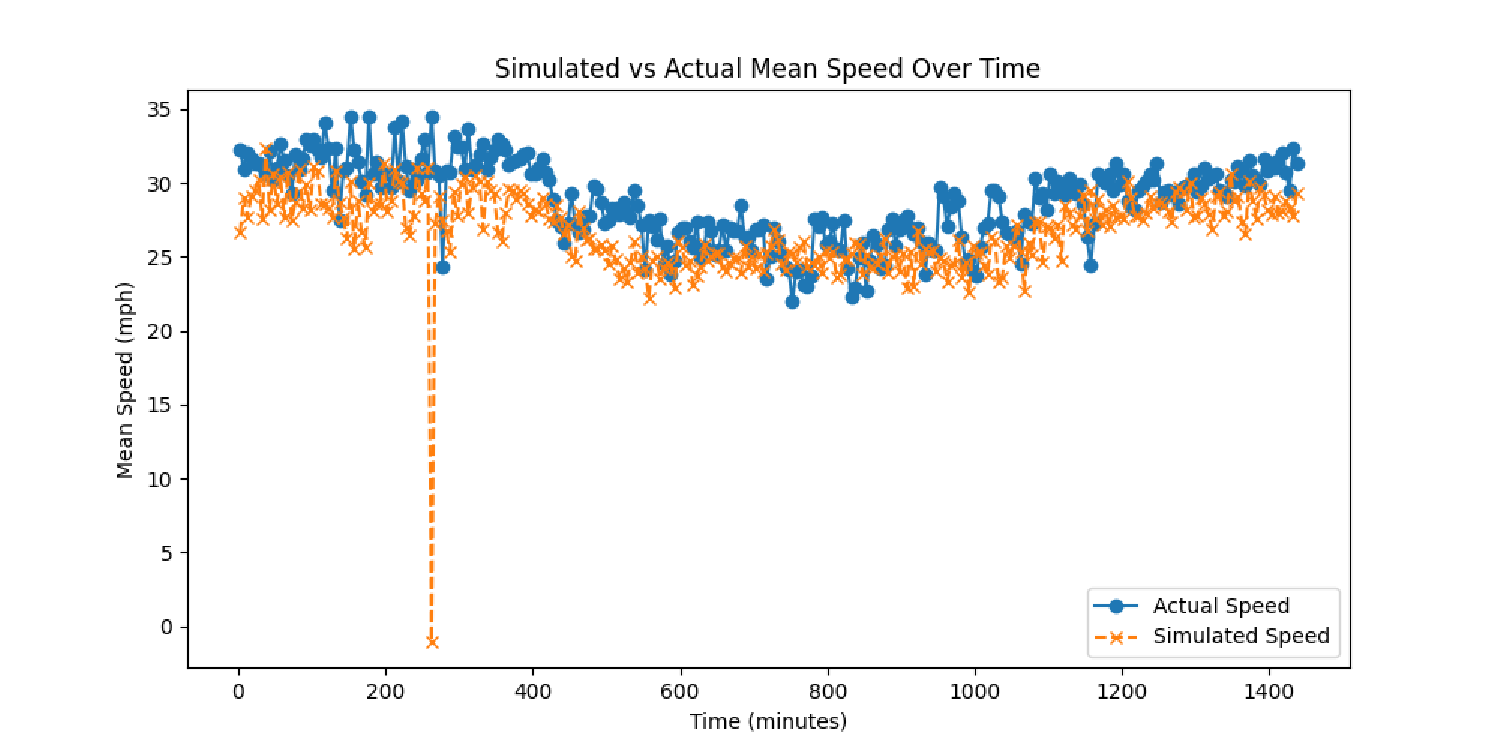
\includegraphics[width=\textwidth]{images/results-discussions/demand-normal.pdf}
  \caption{Plot of simulation-observed traffic speeds compared with the real world for a typical day}
  \label{fig:demand-normal}
\end{figure}

\begin{figure}[!ht]
  \centering
  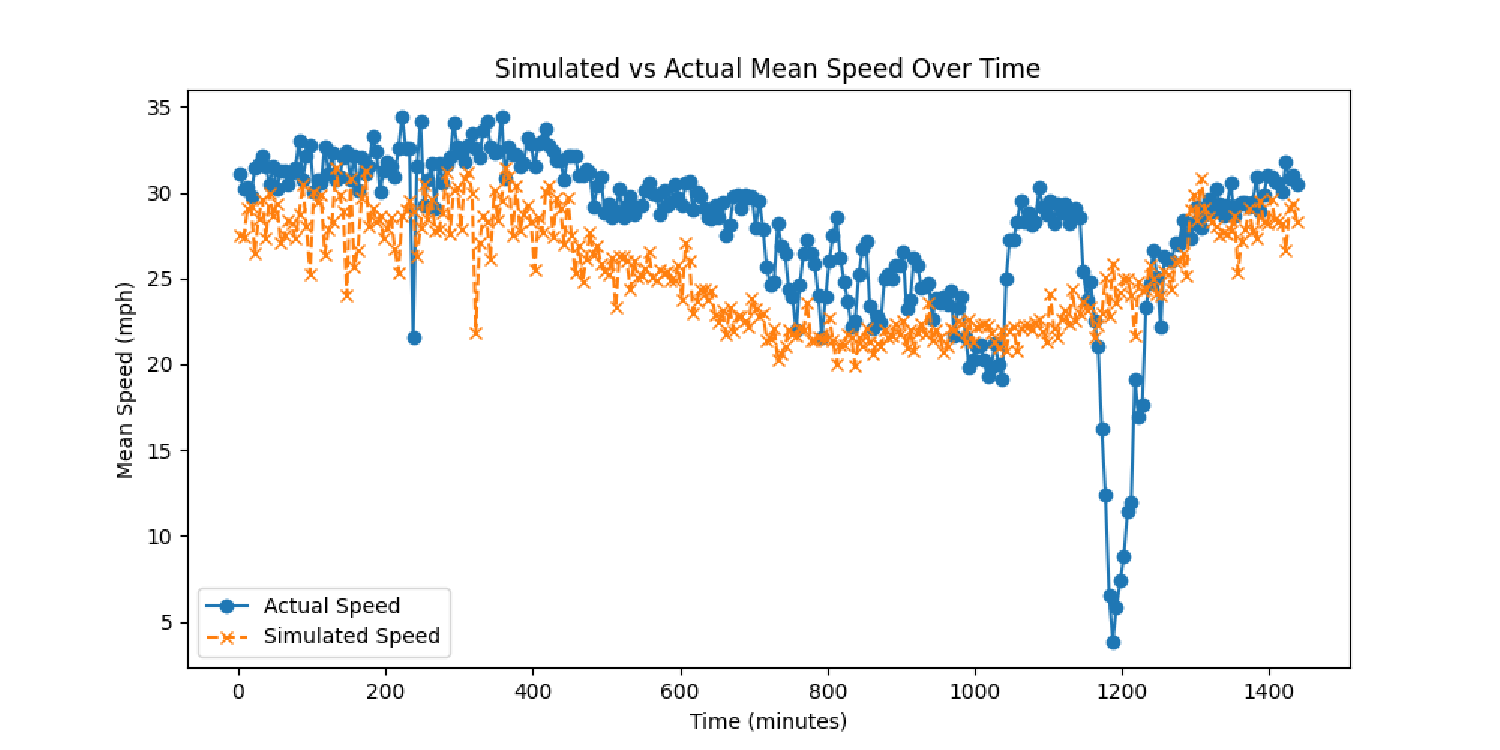
\includegraphics[width=\textwidth]{images/results-discussions/demand-event.pdf}
  \caption{Plot of simulation-observed traffic speeds compared with the real world for an event day}
  \label{fig:demand-event}
\end{figure}

\subsubsection{Reactive Hyperparameter Search}
We cover the results of the hyperparameter search performed on the reactive strategy to choose the best option to simulate against the proactive and baseline strategies. The results are shown in \tab{reactive-bench-results} and \fig{reactive-bench-results}. Since we implemented an optimisation to discard all combinations where the simulation timed out, which discarded all the worst combinations, we are left with all the combinations that perform equally. The results of this rule are further validated by the significant decrease in emissions and a slight decrease in time loss, with a minimal trip duration increase. Since all the options remaining performed equally, we chose the option which had the highest number of individual hyperparameters present among all the options. This resulted in the rule with a High Traffic Threshold (HTT) of 50, Speed Reduction 1 (SR1) of 25 MPH and Speed Reduction 2 (SR2) of 20 MPH, which becomes our reactive rule.

\begin{table}[!ht]
    \centering
    \caption{Reactive Hyperparameter Search Results and Metrics}
    \label{table:reactive-bench-results}
    \resizebox{\textwidth}{!}{%
    \begin{tabular}{lcccccc}
        \toprule
        \textbf{Control Mode} & \textbf{HTT} & \textbf{SR1} & \textbf{SR2} & \textbf{Avg. Trip Duration (s)} & \textbf{Avg. Emissions (g)} & \textbf{Avg. TimeLoss (s)} \\
        \midrule
        Baseline & -- & -- & -- & 212.23 & 3604.93 & 54.41 \\
        reactive\_rule\_ril\_0\_rih\_3\_ti\_0    & 30 & 25 & 10 & 213.63 & 3507.14 & 53.52 \\
        reactive\_rule\_ril\_0\_rih\_3\_ti\_1    & 40 & 25 & 10 & 213.63 & 3507.14 & 53.52 \\
        reactive\_rule\_ril\_0\_rih\_3\_ti\_2    & 50 & 25 & 10 & 213.63 & 3507.14 & 53.52 \\
        reactive\_rule\_ril\_1\_rih\_3\_ti\_2    & 50 & 25 & 15 & 213.63 & 3507.14 & 53.52 \\
        reactive\_rule\_ril\_2\_rih\_3\_ti\_0    & 30 & 25 & 20 & 213.63 & 3507.14 & 53.52 \\
        reactive\_rule\_ril\_2\_rih\_3\_ti\_1    & 40 & 25 & 20 & 213.63 & 3507.14 & 53.52 \\
        reactive\_rule\_ril\_2\_rih\_3\_ti\_2    & 50 & 25 & 20 & 213.63 & 3507.14 & 53.52 \\
        \bottomrule
    \end{tabular}%
    }
\end{table}

\begin{figure}[!ht]
  \centering
  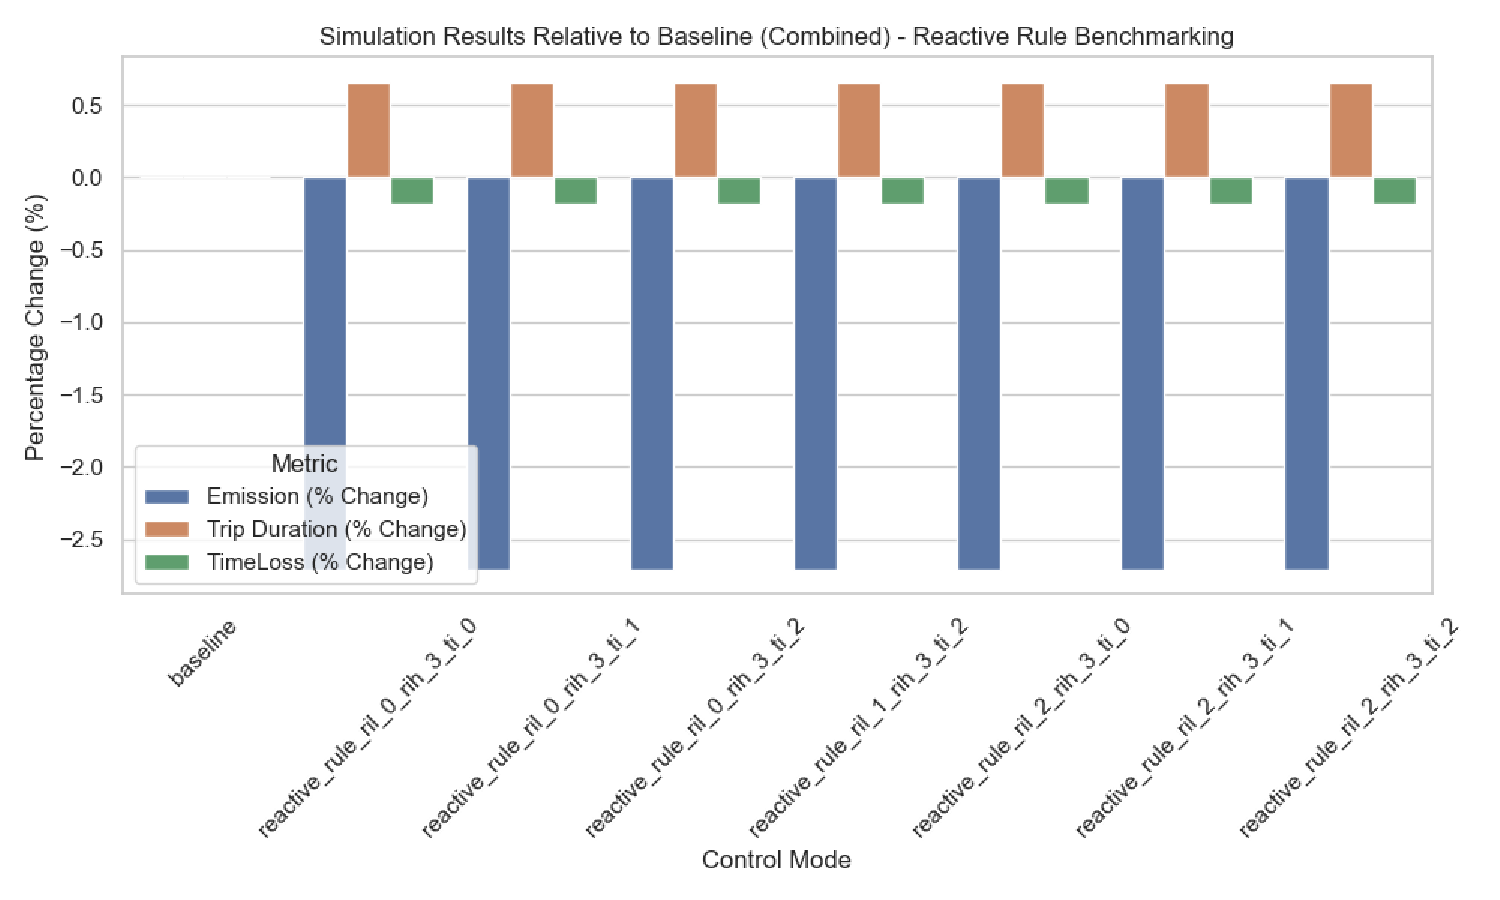
\includegraphics[width=\textwidth]{images/results-discussions/reactive-bench.pdf}
  \caption{Plot of results of hyperparameter optimisation for reactive rule strategy}
  \label{fig:reactive-bench-results}
\end{figure}

\subsubsection{Baseline vs. Reactive vs. Proactive Strategies}
The simulations were run using all the defined strategies on both the 2024 simulations and event-day simulations, as previously discussed. The control modes are self-descriptive; however, to make clear, “predictive” uses the raw model output of speed for that particular timestep, while predictive\_30 uses predictions 30 minutes in advance. The “predictive\_round2” and “predictive\_round5” use the current predictions rounded to the nearest 2 and 5 MPH, respectively. To reduce the number of combinations, the rounding was only tested on the “predictive” mode, as for both simulation rounds, “predictive” obtained better results than “predictive\_30”.

\tab{2024-sims} shows the average results over the whole traffic network tested for the 2024 simulations, while \tab{match-sims} shows the results for the event-day simulations. The tables present the mean and standard deviations for the three metrics we designed to focus on through all the control modes for that particular simulation batch run. We also provide visualisations through plots of the means of the metrics, using the percentage differences from the baseline for a more specific analysis. \fig{2024-sims-full} shows this plot for the 2024 simulations and \fig{event-sims-full} for the event-day simulations. For both of these runs, an outlier control mode resulted in significant congestion compared to all others. For easier interpretation, we have removed these outliers (“predictive\_30” for the 2024 simulations and “lower\_limit” for the event-day simulations) in \fig{2024-sims-reduced} and \fig{event-sims-reduced}, respectively.

\begin{table}[!ht]
    \centering
    \caption{Results of congestion management techniques on 2024 simulations}
    \label{table:2024-sims}
    \resizebox{0.9\textwidth}{!}{%
    \begin{tabular}{lcccccc}
        \toprule
        \multirow{2}{*}{\textbf{Control Mode}} &
        \multicolumn{2}{c}{\textbf{~Avg. Trip Duration (s)~}} &
        \multicolumn{2}{c}{\textbf{~Avg. Trip Emissions (g)~}} &
        \multicolumn{2}{c}{\textbf{~Avg. Trip TimeLoss (s)~}} \\
        & \textbf{~Mean~} & \textbf{~Std. Dev.~} 
        & \textbf{~Mean}~ & \textbf{~Std. Dev.~} 
        & \textbf{~Mean~} & \textbf{~Std. Dev.~} \\
        \midrule
        baseline           & 212.29 & 4.17   & 3576.74 & 886.23  & 53.85  & 4.24   \\
        lower\_limit       & 220.33 & 2.33   & 3909.72 & 573.59  & 53.99  & 2.40   \\
        predictive         & 214.18 & 5.55   & 3410.36 & 764.62  & 54.56  & 5.44   \\
        predictive\_30     & 287.86 & 299.11 & 4983.88 & 6360.49 & 118.11 & 258.47 \\
        predictive\_round2 & 212.90 & 2.54   & 3380.20 & 457.54  & 53.19  & 2.46   \\
        predictive\_round5 & 214.02 & 3.01   & 3578.66 & 715.42  & 53.39  & 2.85   \\
        reactive\_rule     & 212.97 & 2.75   & 3408.62 & 551.42  & 53.11  & 2.60   \\
        \bottomrule
    \end{tabular}%
    }
\end{table}

\begin{table}[!ht]
    \centering
    \caption{Results of congestion management techniques on event-day simulations}
    \label{table:match-sims}
    \resizebox{0.9\textwidth}{!}{%
    \begin{tabular}{lcccccc}
        \toprule
        \multirow{2}{*}{\textbf{Control Mode}} &
        \multicolumn{2}{c}{\textbf{~Avg. Trip Duration (s)~}} &
        \multicolumn{2}{c}{\textbf{~Avg. Trip Emissions (g)~}} &
        \multicolumn{2}{c}{\textbf{~Avg. Trip TimeLoss (s)~}} \\
        & \textbf{~Mean~} & \textbf{~Std. Dev.~} 
        & \textbf{~Mean}~ & \textbf{~Std. Dev.~} 
        & \textbf{~Mean~} & \textbf{~Std. Dev.~} \\
        \midrule
        baseline           & 209.35 & 2.06 & 3553.06 & 513.19 & 51.68 & 1.96 \\
        lower\_limit       & 218.18 & 1.83 & 3960.41 & 427.48 & 52.54 & 1.74 \\
        predictive         & 211.01 & 1.98 & 3359.95 & 404.68 & 51.52 & 1.79 \\
        predictive\_30     & 210.82 & 2.01 & 3488.96 & 424.20 & 51.32 & 1.82 \\
        predictive\_round2 & 211.38 & 2.07 & 3424.87 & 489.96 & 51.66 & 1.86 \\
        predictive\_round5 & 212.12 & 2.30 & 3543.96 & 404.90 & 51.79 & 2.09 \\
        reactive\_rule     & 210.75 & 1.95 & 3526.20 & 415.62 & 51.63 & 1.70 \\
        \bottomrule
    \end{tabular}%
    }
\end{table}

\paragraph{Discussion of Results}
The first important point is that simply setting a lower speed limit as a congestion management technique is ineffective. Both trip duration and emissions largely spike upwards, confirming that the results obtained with the other strategies are not simply due to a lower speed limit.

Secondly, we note that the reactive strategy is effective. For both the 2024 simulation runs and event-day-specific ones, we see that the reactive strategy significantly reduces emissions while only slightly increasing trip duration. The effect of this strategy is much higher for the overall simulations compared to event days. For these, it is still efficient but at a much lower magnitude. This is expected, and we expect the proactive congestion techniques to fill the gap.

Discussing the proactive techniques, we present exciting results. For the 2024 simulations, the pure predictive approach performs just as well as the reactive versions, with a slight increase in trip duration and time loss. However, the predictive technique outperforms its reactive counterpart for event days. Here, the predictive approach achieves reduced emissions of more than 5\% on average, compared to the reactive \~{}0.5\%, as well as a more significant reduction of time loss while keeping similar trip durations. These results prove the potential of proactive congestion management techniques, especially during events.

For the variants with rounding, rounding to the nearest 5 MPH presents disappointing results. However, rounding to the nearest 2 MPH improves the results for the general 2024 simulations and only slightly reduces the effectiveness in the event-day simulations, proving that the predictive approach can outperform typical reactive techniques even when rounding is applied.

However, the most interesting result of the simulations is the use of predictions further in advance. For the 2024 simulations, this resulted in total network congestion, while for event days, it performed relatively well but worse than the base predictive mode. This result is slightly different to our initial expected outcome, for which further work is needed, but we hypothesise the following:
\begin{enumerate}
    \item A typical reactive or real-time predictive technique may work best for normal conditions. For event days with a more erratic speed pattern, a more advanced prediction may be useful.
    \item Advanced predictions of 30 minutes may be too far in advance and cause congestion through a lower speed limit before it occurs, instead of preventing it early.
    \item The predictions from our ML models are not completely accurate to the specific time. This means that the predictive model may predict a speed decrease some minutes in advance or after the actual speed decrease. This variance in the predictions may already be providing the algorithm with enough information in advance to achieve great results, while manually advancing these by 30 minutes may accentuate this error.
\end{enumerate}

When comparing the variance of the results using their standard deviation, we can also see that the best-performing technique (“predictive\_round2”) has a lower or similar variance to both the baseline and the reactive version, showing that it is also a robust technique that presents consistent results across the simulations tested.

\begin{figure}[!ht]
  \centering
  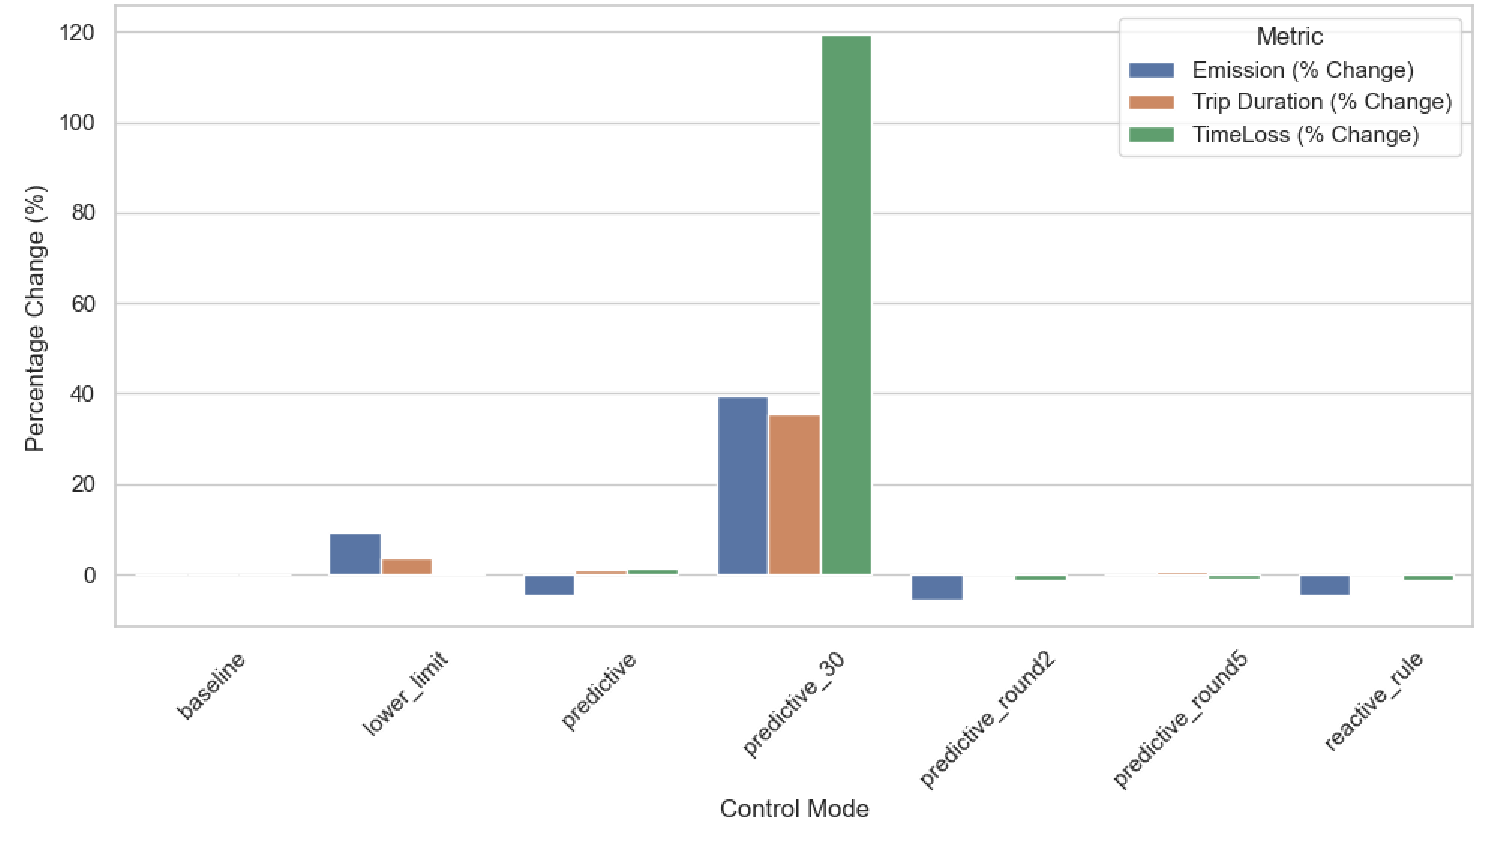
\includegraphics[width=\textwidth]{images/results-discussions/2024-sims-full.pdf}
  \caption{Plot of congestion management techniques results on 2024 simulations}
  \label{fig:2024-sims-full}
\end{figure}

\begin{figure}[!ht]
  \centering
  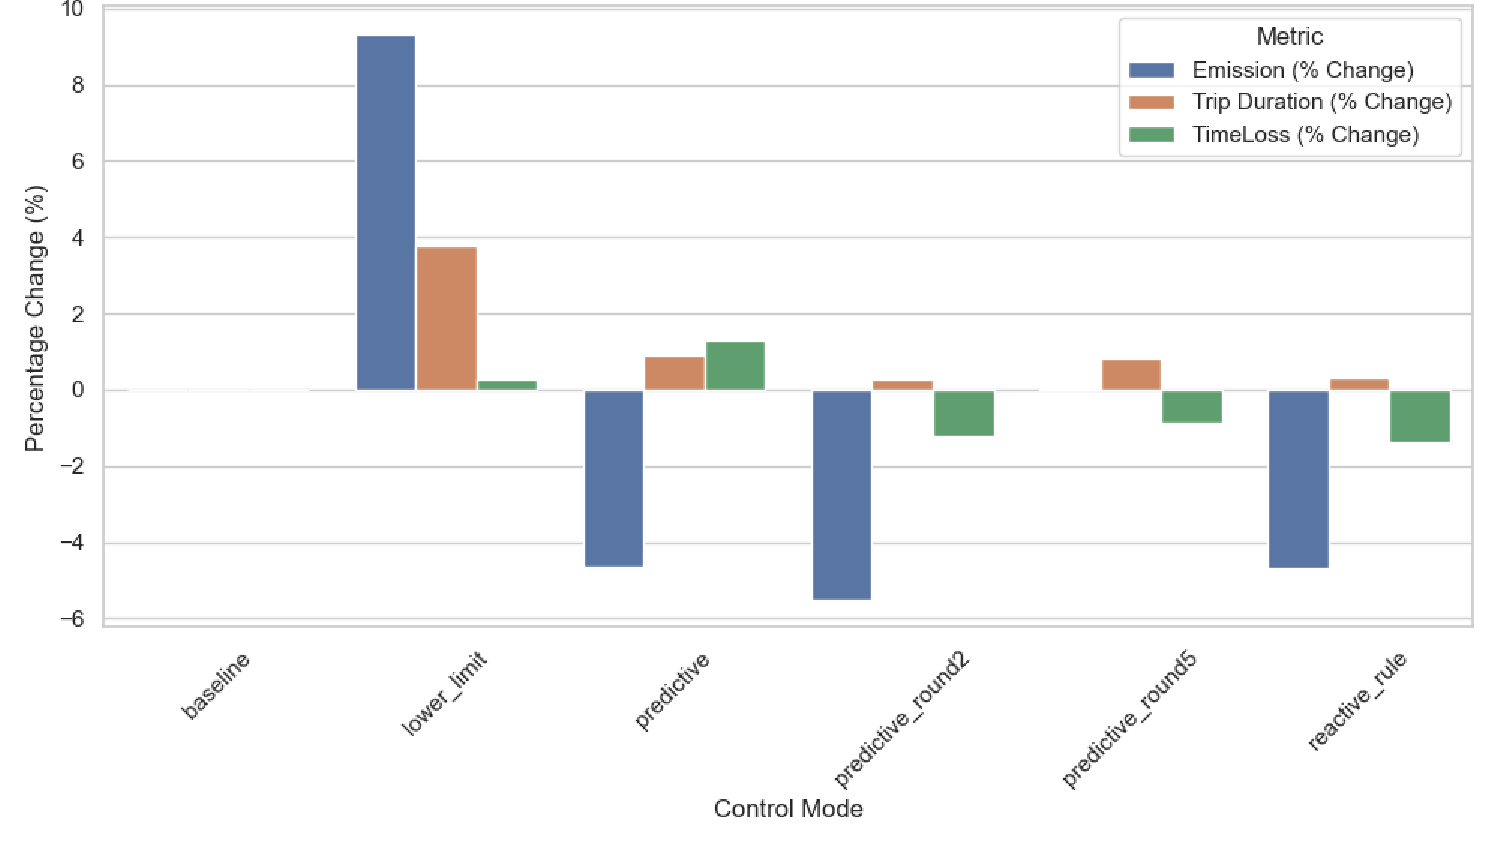
\includegraphics[width=\textwidth]{images/results-discussions/2024-sims-reduced.pdf}
  \caption{Plot of congestion management techniques results on 2024 simulations - outlier removed}
  \label{fig:2024-sims-reduced}
\end{figure}

\begin{figure}[!ht]
  \centering
  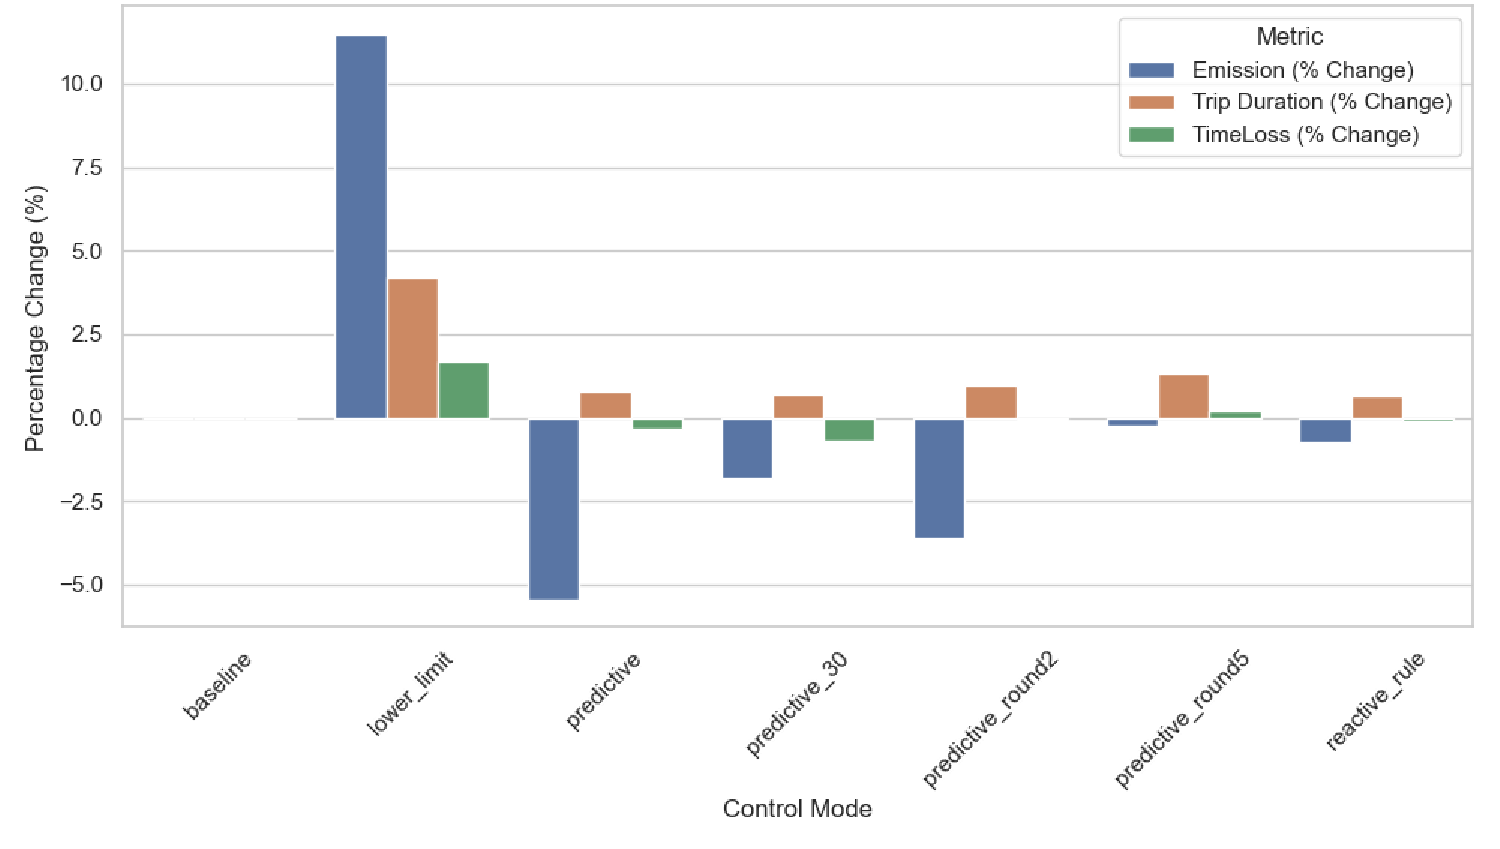
\includegraphics[width=\textwidth]{images/results-discussions/event-sims-full.pdf}
  \caption{Plot of congestion management techniques results on event-day simulations}
  \label{fig:event-sims-full}
\end{figure}

\begin{figure}[!ht]
  \centering
  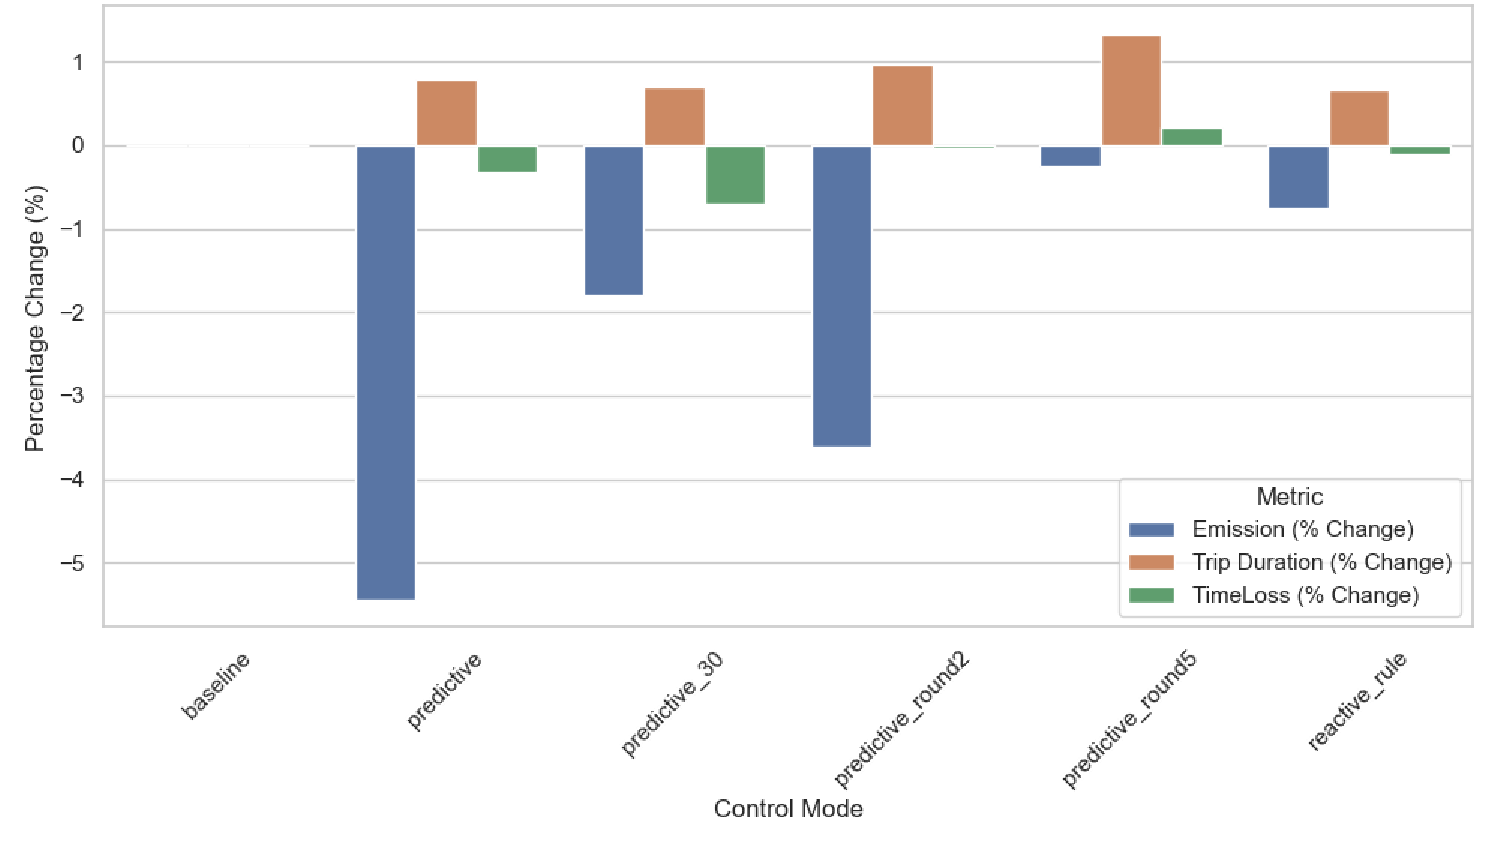
\includegraphics[width=\textwidth]{images/results-discussions/event-sims-reduced.pdf}
  \caption{Plot of congestion management techniques results on event-day simulations - outlier removed}
  \label{fig:event-sims-reduced}
\end{figure}

\subsection{Key Observations}
In summary, a proactive congestion management technique powered by a predictive model can perform far superior to a typical reactive strategy, especially during large-scale events. This technique can significantly decrease congestion, as modelled by the CO\sub{2} emissions reductions and time lost during trips while minimally impacting trip duration. In particular, using the predictions of the exact moment of traffic, coupled with rounding towards the nearest 2 MPH, shows these results while allowing for real-world deployment.

\subsection{Limitations and Sources of Error}
This section briefly discusses the limitations and sources of error for the results presented above. These should be taken into account when analysing the results.

\paragraph{Data Scarcity} The data collected for events and traffic is limited. Therefore, our results are based on this available data, which may not be fully representative of real-world traffic networks. Missing event data can be seen in the earlier model plots, where our predictive model can predict the slower speeds for events it knows about, but many other drops we can not account for are seen. While adding more event data should only improve our algorithms’ accuracy, including more traffic data may alter the simulation outcomes. In collaboration with traffic authorities, traffic data could be severely improved.

\paragraph{Data Variability} Event data is regularly changing, cancelled, or rescheduled. This data needs to be continuously fed into the predictive model for an accurate model.

\paragraph{Simulation using Vehicle Count} As previously discussed, demand generation using vehicle count does not fully represent the actual speeds, especially during events. This lack of representation in the simulations may affect the performance of the algorithms. In theory, if these could be modelled into the simulation demand, it should improve the performance of proactive methods as the actual demand will be closer to the predictive model’s drops.
\end{document}
